\section{Einführung}
% \paragraph{Logical- und Visual-Tree}
% Der \textbf{Logical Tree} enstpricht der Struktur der XAML Elemente. Es beschreibt Beziehungen zwischen verschiedenen Elementen des UIs. Der \textbf{Visual Tree} entspricht der grafischen Repräsentation und beinhaltet alle dargestellten Elemente gemäss der Vorlage jedes Controls. \\
% 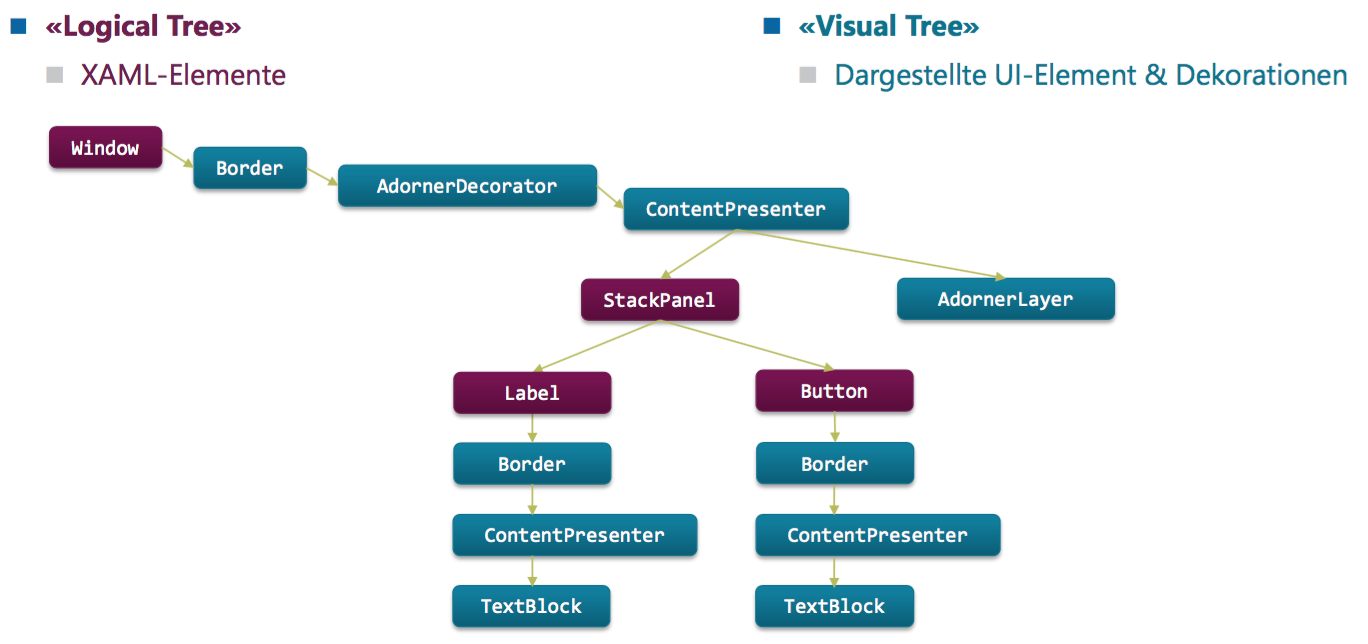
\includegraphics[scale=0.27]{LogicalVisual.png}
% Der Logical-Tree entspricht der Strukutr der XAML-Elemente. Sie beschreibt die Beziehungen zwischen verschiedenen Elementen des UI. Es ist Zuständig für:
% \begin{itemize}
%     \item Dependency Properties erben
%     \item Dynamische Ressourcen-Referenzen auflösen
%     \item Elementnamen für Datenbindung nachschlagen
%     \item Routed Events weiterleiten
% \end{itemize}
% Der Visual-Tree entspricht der grafischen Repräsentation und beinhaltet alle dargestellten Elemente gemäss der Vorlage jedes Controls. Es ist Zuständig für:
% \begin{itemize}
%     \item Visuelle Darstellung
%     \item Vererben der Transparenzeinstellungen
%     \item Vererben von Transformationen
%     \item Vererben der IsEnabled-Property
%     \item Hit-Testing
% \end{itemize}
\paragraph{Syntax}
\textbf{Attribute Syntax}
\begin{lstlisting}[language=xml]
<Button Height="50" Width="200" Content="Watch Now" />
\end{lstlisting}
\textbf{Property Element Syntax}
\begin{lstlisting}[language=xml]
<Button Width="120" Height="50"
  <Button.Content>Watch Now</Button.Content>
</Button>>
\end{lstlisting}
Mit dem Property Element Syntax ist zusammengesetzter Inhalt möglich. 
\begin{lstlisting}[language=xml]
<Button Height="50" Width="200" Content="Watch Now" />

<Button Width="120" Height="50">
  <Button.Content>Watch Now</Button.Content>
</Button>

<Button Width="120" Height="50">
  <Button.Content>
    <StackPanel>
     <TextBlock Text="Watch Now" FontSize="20" />
     <TextBlock Text="Duration: 50m" FontSize="12" 
        Foreground="#888888" />
    </StackPanel>
  </Button.Content>
</Button> 
\end{lstlisting}

\paragraph{Projekt-Layout}
\begin{description}
    \item[App.config] Config-File mit App-Einstell., Connection Strings, etc.
    \item[App.xaml] Markup der Startup-Klasse
    \item[App.xaml.cs] Code-Behind der Startup Klasse
    \item[MainWindow.xaml] Markup des Hauptfensters
    \item[MainWindow.xaml.cs] Code-Behind des Hauptfensters
\end{description}

\section{Layout und Controls}

\paragraph{App \& Window}
App.xaml + App.xaml.cs + App.g.cs $\Rightarrow$ globale Application-Klasse App \\
Code Generator erzeugt App.g.cs im obj Verzeichnis, diese beinhaltet globale Main-Methode $\Rightarrow$ Einstiegspunkt der App
\begin{lstlisting}[language=xml]
<Application x:Class="HelloWpf.App"
             xmlns="http://schemas.microsoft.com/winfx/2006/xaml/presentation"
             xmlns:x="http://schemas.microsoft.com/winfx/2006/xaml"
             xmlns:local="clr-namespace:HelloWpf" 
             StartupUri="MainWindow.xaml">
    <Application.Resources>...</Application.Resources>
</Application>
\end{lstlisting}

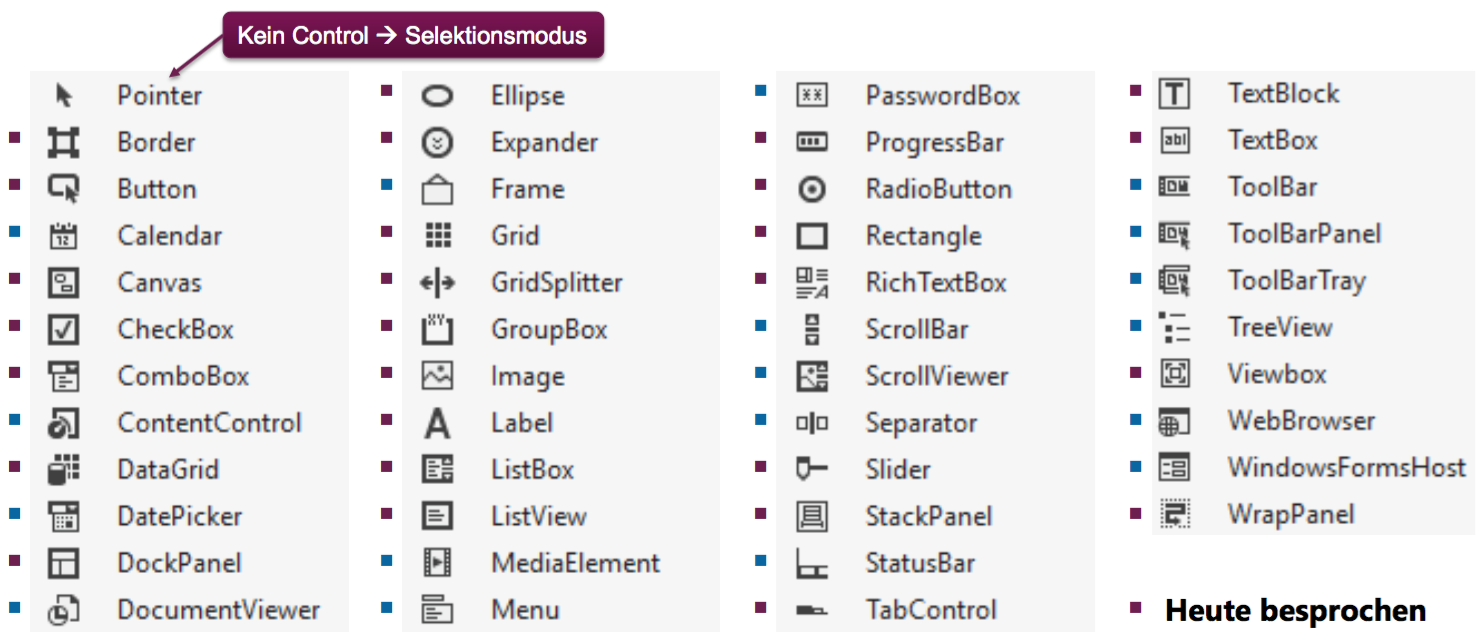
\includegraphics[scale=0.25]{ControlsOverview.png}

\paragraph{Window-Definition}
\begin{lstlisting}[language=xml]
<Window xmlns="http://schemas.microsoft.com/winfx/2006/xaml/presentation" xmlns:x="http://schemas.microsoft.com/winfx/2006/xaml" xmlns:local="clr-namespace:Assignment1.Mvvm.App" x:Class="HelloWpf.MainWindow« Title="AutoWindow" ... > 
<!-- Client area (for content) --> 
</Window>
\end{lstlisting}
\begin{description}
    \item[Standardnamespace] WPF Control Library (WPF-Klassen als XML-Tags ohne Präfix nutzbar)
    \item[XML Namespace x] XAML-spezifische Definition (Angaben mit x:-Präfix nutzbar)
    \item[XML Namespace local] macht C#-Namespace verfügbar (Klassen mit local:-Präfix nutzbar)
\end{description}

\paragraph{Grössenangaben} Zur Manipulation von Width und Height Attributen (\code{System.Windows.FrameworkElement}) kann man fixe Grössenangaben verwenden, diese werden als \code{double} Werte geschrieben. Wenn kein Kennzeichner angegeben ist (nur eine Zahl), wird automatisch \textit{Device Independent Pixel} verwendet $\left(\frac{1}{96}''\right)$. Qualfizierte Grössenangaben sind:
\begin{itemize}
\item \textbf{px} Device Independent Pixels $\left(1\text{px} = \frac{1}{96}''\right)$
\item \textbf{in} Inches (Zoll) $1\text{in} = 96\text{px}$
\item \textbf{cm} $1\text{cm} = \frac{96}{2.54}\text{px}$
\item \textbf{pt} Points $1\text{pt} = \frac{1}{72}'' = \frac{96}{72}\text{px}$
\end{itemize}
Zusätzlich kann man noch \code{MinWidth} und \code{MaxWidth} definieren. Bei Platzproblemen wird zuerst MinWidth, dann MaxWidth und dann Width evaluiert. Das Read-only Property \code{ActualWidth} kann verwendet werden um die Fenstergrösse während der Laufzeit abzufragen. 


\paragraph{Ausrichtung} HorizontalAlignment und VerticalAlignment Attribute manipulieren die Ausrichtung innerhalb des Containers. Es gibt auch HorizontalContentAlignment und VerticalContentAlignment für Inhaltsaurichtung beispielsweise für TextBox. \\
Valide Werte sind: Left, Center, Right und Stretch für Horizontal bzw. Top, Center, Bottom und Stretch für Vertical. Stretch füllt jeweils die komplette Verfügbare Achse. \textbf{Stretch hat jeweils eine tiefere Priorität als fixe Width/Height-Angaben!}
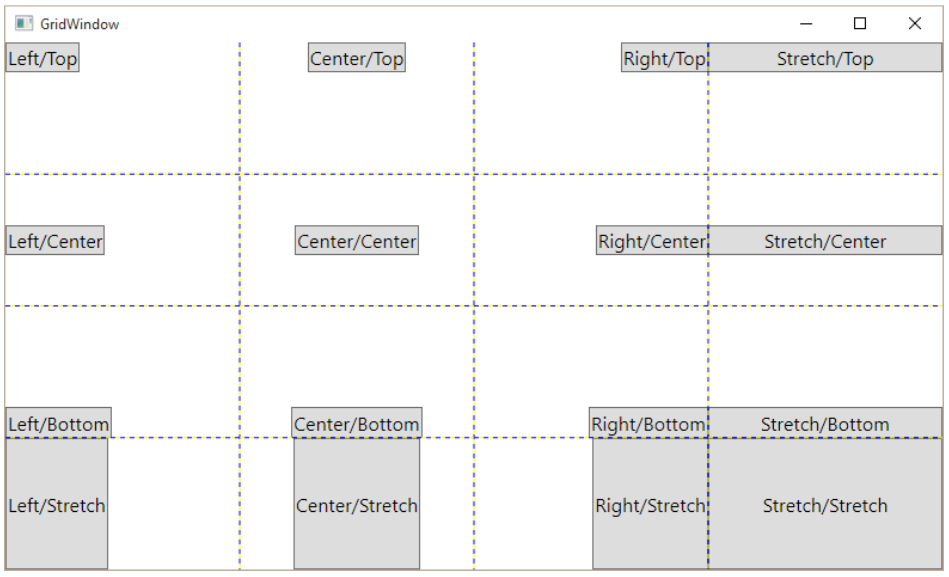
\includegraphics[scale=0.25]{img/ausrichtung.png}


\paragraph{Ränder \& Rahmen} Um Rahmengrössen anzupassen gibt es:
\begin{description}
    \item[Margin] = Aussenabstand
    \item[Padding] = Innenabstand
    \item[BorderThickness] = Rahmenstärke
    \item[CornerRadius] = Radius für abgerundete Ecken beim Rahmen
\end{description}
Folgende Werte sind zulässig:
\begin{itemize}
\item \textbf{l,t,r,b}
\item \textbf{l,t} Left=Right, Top=Bottom
\item \textbf{x} Auf allen Seiten gleich viel Abstand
\end{itemize}
Bei Corner Radius gibt es nur eine zulässige Definition:
\begin{itemize}
\item TopLeft, TopRight, BottomRight, BottomLeft
\end{itemize}
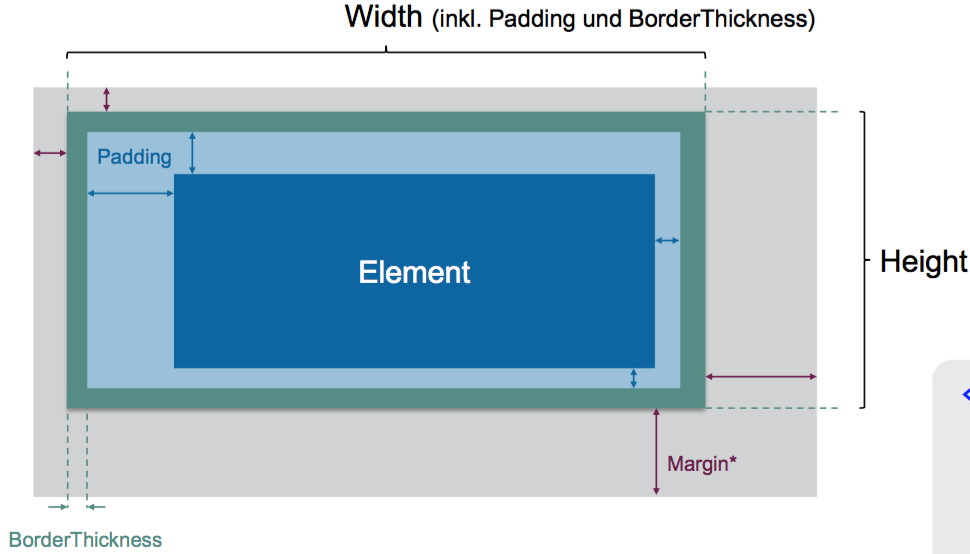
\includegraphics[scale=0.35]{Rahmen.png}
\begin{lstlisting}[language=xml]
<Button Width="100" Height="60" BorderThickness="4" Margin="10,10,40,40" Padding="30,20,10,10" Content="Element" /> 
\end{lstlisting}
Folgende Anwendungen gibt es zusätzlich: \\
\textbf{UIElement}
\begin{itemize}
    \item \code{IsEnabled}
    \item \code{SnapsToDevicePixels} (Rundet Pixelangaben auf physikalische Gerätepixelwerte)
    \item \code{Visibility} (Collapsed, Hidden, Visible)
\end{itemize}
\textbf{FrameWorkElement}
\begin{itemize}
    \item \code{Name} = Name des Elements (u.a für Code-Behind)
    \item \code{Resource} = Lokal definierte Ressourcen 
    \item \code{Tag} = Wert zur Markierung
    \item \code{Tooltip} = Setzt den Tooltip
    \item \code{UseLayoutRounding} = Rundet Layout-Pixelangaben auf physische Gerätepixelwerte (Standard = false)
\end{itemize}
\textbf{Control}
\begin{itemize}
    \item \code{Background} = Brush für Hintergrund
    \item \code{BorderBrush} = Brush für Rahmen
    \item \code{Foreground} = Brush für Schrift
    \item \code{FontFamily} = Schriftartfamilie
    \item \code{FontSize} = Schriftgrösse
    \item \code{FontStretch} = UltraCondensed, Normal, UltraExpanded
    \item \code{FontStyle} = Normal, Italic, Oblique
    \item \code{FontWeight} = ExtraBold, Bold, SemiBold, Normal, Light, ExtraLight
\end{itemize}
\textbf{Schrifteinstellungen inkl. Brush} werden an Child Controls vererbt, sonstiges i.d.R nicht.


\paragraph{Brush} Mit Brushes kann man einfache oder komplexe Farbverläufe darstellen. Es gibt 6 Pinseltypen
\begin{itemize}
    \item \code{SolidColorBrush} (Einfarbig)
    \item \code{LinearGradientBrush} (Einfacher Farbverlauf)
    \item \code{RadialGradient} Farbverlauf (Runder Farbverlauf, errinert an Kugel)
    \item \code{ImageBrush} (Bild innerhalb des Brushes)
    \item \code{DrawingBrush} (Spezielle Muster)
    \item \code{VisualBrush} (Komplexte Textdarstellung)
\end{itemize}

\begin{lstlisting}[language=xml]
<Button Name="GoButton" Content="Go" Background="Black" />
<Button Name="GoButton" Content="Go" Background="#000000" />
<Button Content="Go">
  <Button.Background>
    <SolidColorBrush Color="Black" />
  </Button.Background>
</Button>

<Button ...>
  <Button.Background>
    <SolidColorBrush>
      <SolidColorBrush.Color>
        <Color R="128" G="156" B="255" A="128" />
      </SolidColorBrush.Color>
    </SolidColorBrush>
  </Button.Background>
</Button> 
\end{lstlisting}

\begin{lstlisting}[language=java]
GoButton.Background = Brushes.Black;
GoButton.Background = new SolidColorBrush(Colors.Black);
\end{lstlisting}

\paragraph{Clipping} Mit \code{ClipToBounds="True"} kann man definieren, ob Child Controls an den Rändern des Parent Controls abgeschnitten werden sollen. Mit \code{Clip} kann man definieren welche Form zum Zuschneiden eines Controls verwendet werden soll.
\begin{lstlisting}[language=xml]
<Image.Clip>
    <EllipseGeometry
        RadiusX="100"
        RadiusY="75"
        Center="100, 75" />
</Image.Clip>
\end{lstlisting}
\subsection{Container Controls} Bei Container gibt es welche mit Layout und ohne Layout. Container mit Layout sind: \textbf{StackPanel}, \textbf{WrapPanel} (Umbruch erfolgt anhand Objektbreite, kein fixer unterer Randabstand möglich), \textbf{DockPanel} und \textbf{Grid}. Container ohne Layout sind: \textbf{Canvas}, \textbf{ScrollViewer}, \textbf{Viewbox} und \textbf{Border}.

\paragraph{StackPanel}
\begin{itemize}
    \item \code{Attribut=Horizontal/Vertical}, definiert die \textbf{Anordnung} der Elemente
    \item kein fixer unterer Randabstand möglich
    \item Füllt leeren Platz nicht aus $\Rightarrow$ \textbf{nicht für Responsives Design geeignet}
\end{itemize}

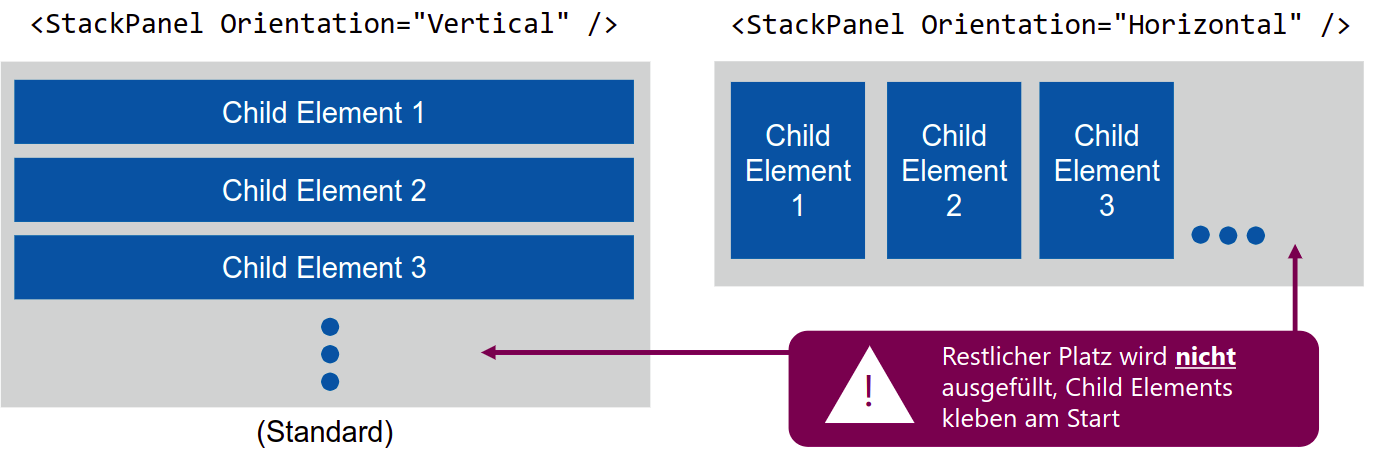
\includegraphics[scale=0.18]{img/stackpanel-overview.png}

\paragraph{WrapPanel} Wie StackPanel aber mit Zeilen-/Spaltenumbruch. 


\paragraph{DockPanel}
\begin{itemize}
    \item \code{DockPanel.Dock} definiert, wo der Container sein wird
    \item Verfügbare Platz wird in absteigender Reheinfolge verteilt
    \item Letztes definiertes Child Element füllt verbleibenden Platz aus
    \item Mit \code{LastChildFill = False} füllt das letzte Element den Platz nicht mehr aus.
\end{itemize}
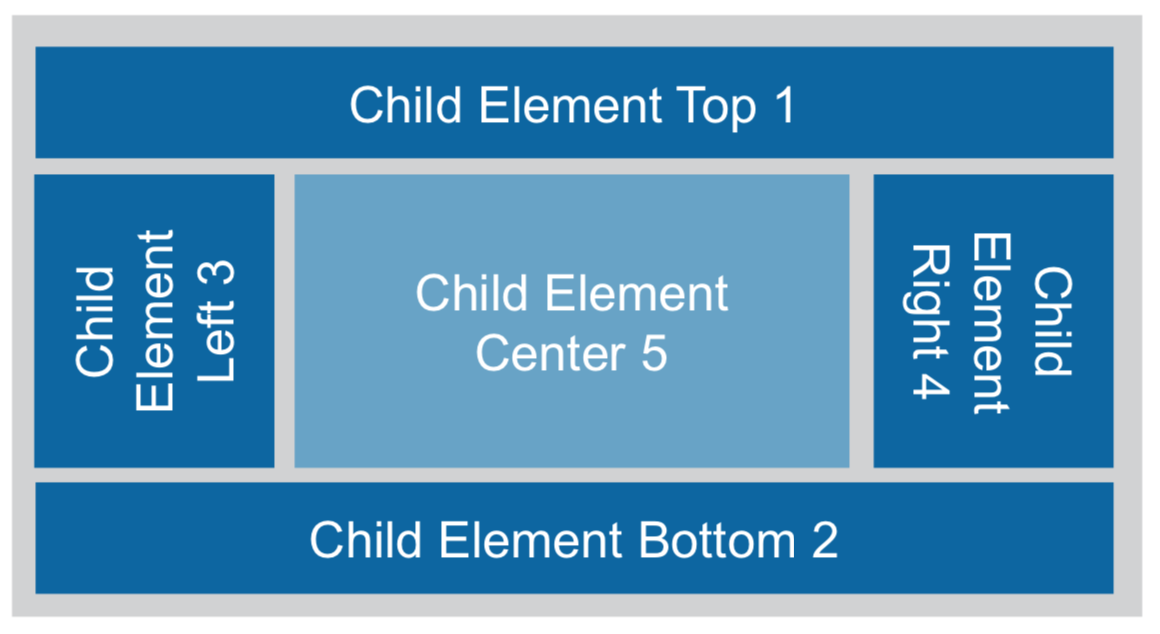
\includegraphics[scale=0.2]{DockPanel.png}
\begin{lstlisting}[language=xml]
<DockPanel> 
  <TextBlock Text="Child Element Top 1" 
      DockPanel.Dock="Top" /> 
  <TextBlock Text="Child Element Bottom 2" 
      DockPanel.Dock="Bottom" /> 
  <TextBlock Text="Child Element Left 3" 
      DockPanel.Dock="Left" /> 
  <TextBlock Text="Child Element Right 4" 
      DockPanel.Dock="Right" /> 
  <TextBlock Text="Child Element Center 5" /> 
</DockPanel>
\end{lstlisting}
Reihenfolge wichtig. Hier top erstes Child.
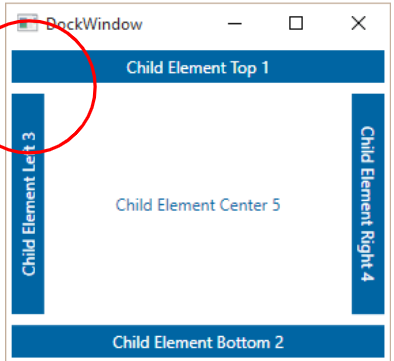
\includegraphics[scale=0.3]{img/dockpanelbeispiel.png}


\paragraph{Grid} 
Row = waagerecht. Column = senkrecht. 
Anzahl Spalten und Zeilen müssen zuerst definiert werden (siehe Beispiel unten) 
\begin{description}
    \item[Ganzzahlen] Fixe Breite/Höhe
    \item[Auto] Nur benötigter Platz 
    \item[*] Proportionale Aufteilung des verfügbaren Rest-Platzes 
    \item[2*] Rest-Platz wird gewichtet (Ganzahl vor *) aufgeteilt (Workaround, da keine Prozent erlaubt)
    \item[MinWidth/MinHeight und MaxWidth/MaxHeight]
\end{description}

\begin{lstlisting}[language=xml]
<Grid>
    <Grid.ColumnDefinitions>
        <ColumnDefinition></ColumnDefinition>
        <ColumnDefinition></ColumnDefinition>
        <ColumnDefinition></ColumnDefinition>
    </Grid.ColumnDefinitions>
    <Grid.RowDefinitions>
        <RowDefinition></RowDefinition>
        <RowDefinition></RowDefinition>
        <RowDefinition></RowDefinition>
    </Grid.RowDefinitions>
</Grid>
\end{lstlisting}
Mit \code{RowSpan} bzw. \code{ColumnSpan} möglich, Elemente über mehrere Zellen/Spalten zu strecken. \\
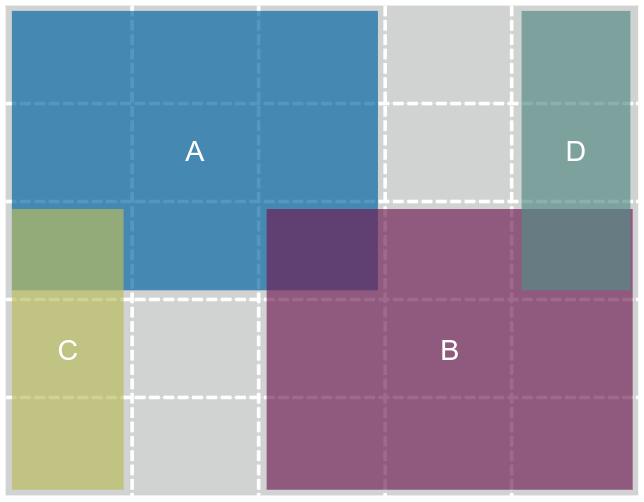
\includegraphics[scale=0.3]{img/rowspancolspan.png}
\begin{lstlisting}[language=xml]
<Grid>
    <Grid.ColumnDefinitions>...</Grid.ColumnDefinitions>
    <Grid.RowDefinitions>...</Grid.RowDefinitions>
    <Button Content="A"
        Grid.Column="0" Grid.Row="0"
        Grid.RowSpan="3" Grid.ColumnSpan="3" />
    <Button Content="B"
        Grid.Column="2" Grid.Row="2"
        Grid.RowSpan="3" Grid.ColumnSpan="3" />
    <Button Content="C"
        Grid.Column="0" Grid.Row="2"
        Grid.RowSpan="3" Grid.ColumnSpan="1" />
    <Button Content="D"
        Grid.Column="4" Grid.Row="0"
        Grid.RowSpan="3" Grid.ColumnSpan="1" />
</Grid>
\end{lstlisting}
\textbf{Stapelung} Bei einem 1 x 1 Grid werden die Elemente in der Zelle gestapelt und man kann mit Alignments und Margin ein flexibles Layout erstellen.
%  Das ist weiter unten zu finden:
%\paragraph{Application}
% \begin{description}
%     \item[Current]: Statischer Zugriff auf die Anwndungsklasse (Singleton). Beispiel  \code{public App MyApp => Application.Current as App; }
%     \item[ShutdownMode]: Verschiedene Shutdown Modi: \code{OnLastWindowClose} App wird beim Scliessen des letzten Fensters beendet (Standard). \code{OnMainWindowClose} App wird beendet sobald Hauuptfenster geschlossen wird. \code{OnExplicitShutdown} App beendet erst, wenn die Shutdown()-Methode aufgerufen wird.
%     \item[StartupUri] Der Name der UI Ressource, welche beim Start geladen/angezeigt werden soll.
%     \item[Windows] Auflistung aller instanziierter Fenster (Window-Objekte) in der App
%     \item[Methoden] \code{public static object LoadComponent(Uri uri)} lädt eine XAML Ressource. \code{public object FindResource(object resourceKey)}sucht Ressource. \code{public void Shutdown(int exitCode)} beender die App und gibt optional den Exit Code an System zurück.
% \end{description}

% \paragraph{Canvas} In einem Canvas Control haben alle Elemente eine absoulte Positionierung und es gibt keine Layout Logik. Die Position innerhalb des Canvas kann mittels \textbf{Attached Properties} festgelegt werden:
% \begin{itemize}
% \item \code{Canvas.Left}: Abstand vom linken Rand
% \item \code{Canvas.Top}: Abstand vom oberen Rand
% \item \code{Canvas.Right}: Abstand vom rechten Rand
% \item \code{Canvas.Bottom}: Abstand zum unteren Rand
% \item \code{Canvas.ZIndex}: Z-Position (Ebene) im Canvas
% \end{itemize}
% In Verbindung mit \code{Shapes} ist ein Canvas Control gut zum "{}programmierten Zeichnen"{} geeignet.
% \begin{lstlisting}[language=xml]
% <Canvas>
%     <Rectangle
%         Canvas.Left="80" Canvas.Top="60"
%         Width="128" Height="80"
%         Fill="#006aa6" />
%     <Ellipse
%         Canvas.Left="260" Canvas.Top="160"
%         Width="120" Height="120"
%         Fill="#6E1C50" />
%     <Path
%         Canvas.Left="120" Canvas.Top="64"
%         Width="260" Height="200"
%         Stroke="DarkGray" Stretch="Fill"
%         Data="M1,0 L0,1"/>
% </Canvas>
% \end{lstlisting}

% \paragraph{Shapes} Die Shapes Klasse beinhaltet \code{Ellipse}, \code{Polygon}, \code{Line}, \code{Polyline}, \code{Path} und \code{Rectangle}. Alle Shapes haben folgende Attribute:
% \begin{itemize}
% \item \textbf{Fill:} Brush für die Füllung
% \item \textbf{Stroke:} Pen für Rahmen/Pinselstrich
% \item \textbf{StrokeThickness:} Breite des Rahmens/Pinselstrichs
% \item \textbf{StrokeDasharray:} Muster für gestrichelte Linien
%     \subitem \textbf{"{}2 1"{}} ist das Verhätniss zwischen Linie/Lücke immer 2:1
%     \subitem \textbf{"{}2 1 4 1"{}} ist das Verhältniss zuerst 2:1, dann 4:1 dann 2:1 etc.
% \item \textbf{StrokeLineJoine:} Art des Übergangs bei Ecken
%     \subitem \textbf{Miter:} Spitzer Rand
%     \subitem \textbf{Bevel:} Abgeschnittener Rand
%     \subitem  \textbf{Round:} Abgerundeter Rand
% \end{itemize}
\paragraph{ViewBox} Skaliert, mittels Transformation, ein einzelnes Child Control um den Verfügbaren Platz auszunutzen. Das Attribut \code{Strech} kann verwendet werden um zu definieren wie das Control skaliert werden soll. Valid sind: \code{None} (keine Skalierung), \code{Uniform} (Vergrössern bis es ins Controll passt), \code{Fill} (Strecken, dass kompletter Platz verwendet wird), \code{UniformToFill} (Vergrössern und Strecken, dass Proportionen erhalten bleiben, aber ganzes Control ausgefüllt wird. Bei Übergrösse wird das Alignment berücksichtigt.
\paragraph{Border} Die Border zeichnet lediglich ein Rahmen um ein Child Control. Es kann mit Panels kombiniert werden.
\begin{lstlisting}[language=xml]
<Border Background="GhostWhite" CornerRadius="8,0,8,0"
        BorderBrush="#ddd" BorderThickness="1"
        Margin="10"
        Padding="10">
    <StackPanel Orientation="Vertical">
        <Button Margin="0,0,0,5" Content="Dock Sample 1" />
        <Button Margin="0,0,0,5" Content="Dock Sample 2" />
        <Button Margin="0,0,0,5" Content="Grid Sample 1" />
        <Button Margin="0,0,0,5" Content="Grid Sample 2" />
        <Button Margin="0,0,0,5" Content="Grid Sample 3" />
        <Button Margin="0,0,0,5" Content="Canvas Sample 3" />
    </StackPanel>
</Border>
\end{lstlisting}





\subsection{Input Controls}
\paragraph{Texteingabe}
\begin{description}
    \item[TextBox] Normaler Text Input, mit Option für mehrzeilige Eingabe
    \item[RichTextBox] Text Input mit Formatierung
    \item[PasswordBox] Text wird versteckt
\end{description}
\begin{lstlisting}[language=xml]
<TextBox>Dies ist eine einzeilige TextBox</TextBox> 
<PasswordBox Password="geheim"></PasswordBox> 
<TextBox SpellCheck.IsEnabled="True" AcceptsReturn="True" 
   TextWrapping="Wrap">Das ist eine ...</TextBox> 
<TextBox AcceptsReturn="True" TextWrapping="Wrap" 
   VerticalScrollBarVisibility="Visible">Und das ist ...</TextBox> 
<RichTextBox AcceptsReturn="True" VerticalScrollBarVisibility="Visible"> 
   <FlowDocument> <Paragraph Margin="0"> 
   Und zuletzt noch eine RichTextBox, die auch <Bold>formatierte Inhalte</Bold> darstellen kann. </Paragraph> <Paragraph Margin="0,5"> Dies funktioniert auf Basis der Klasse 
   <TextBlock Foreground="Red" FontWeight="Bold">FlowDocument</TextBlock> und deren <TextBlock Foreground="Blue" FontStyle="Italic">Child Controls</TextBlock>. </Paragraph> </FlowDocument>
</RichTextBox> 
\end{lstlisting}
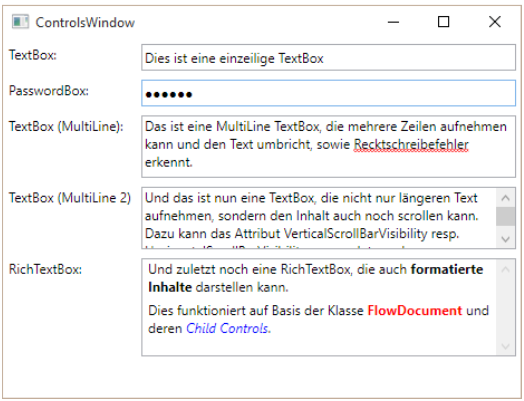
\includegraphics[scale=0.4]{img/texteingabe.png}



\paragraph{Buttons}
\begin{description}
    \item[Button, RadioButton, Checkbox]
    \item[RepeatButton] Löst Click-Event wiederholt aus, bis Button losgelassen wird
    \item[ToggleButton] hat zwei Zustände (Ausgewählt oder nicht). \textbf{Ist Basisklasse für Checkbox und RadioButton.}
\end{description}
\code{isChecked="True"} bedeutet, dass ToggleButton/RadioButton/CheckBox angewählt ist.

\subsection{List Control}
\paragraph{ListBox}
Die \code{ListBox} ist eine komplett sichtbare (scrollable) Liste mit Daten. Diese Einträge können auch Formatierungen beinhalten. 
\begin{description}
    \item[Selection Modes] Single (default), Multiple, Extended
\end{description}
\begin{lstlisting}
<ListBox SelectedIndex="1" SelectionMode="Multiple">
    <ListBoxItem>Erster Eintrag</ListBoxItem>
    <ListBoxItem>Zweiter Eintrag</ListBoxItem>
    <StackPanel Orientation="Horizontal">
        <Rectangle Width="10" Height="10" Fill="Blue" />
        <TextBlock Margin="10,0">Dritter Eintrag</TextBlock>
    </StackPanel>
</ListBox>
\end{lstlisting}

\paragraph{ItemTemplate}
In einer ListBox festlegen, wie die Items angezeigt werden sollen
\begin{lstlisting}
<DataTemplate x:Key="myTaskTemplate" DataType="local:Task">
    <DockPanel HorizontalAlignment="Stretch">
        <TextBlock Text="{Binding TaskName}" />
        <TextBlock Text="{Binding Description}" />
        <TextBlock Text="{Binding Priority}" />
    </DockPanel>
</DataTemplate>

<ListBox ItemSource="{Binding Source={Static Resource myTodoList}}"
    ItemTemplate="{StaticResource myTaskTemplate}" />
\end{lstlisting}

\paragraph{ComboBox} 
\begin{itemize}
    \item \code{IsEditable}
    \item \code{IsReadOnly}
\end{itemize}
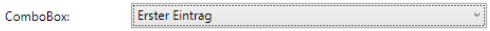
\includegraphics[scale=0.4]{img/ComboBox.png}
\begin{lstlisting}[language=xml]
<ComboBox SelectedIndex="0">
    <ComboBoxItem>Erster Eintrag</ComboBoxItem>
    <ComboBoxItem>Zweiter Eintrag</ComboBoxItem>
</ComboBox>
\end{lstlisting}
\begin{description}
    \item[ListView] Read-Only DataGrid, generalisierte Anzeige einer Liste (Explorer Ansichten)
    \item[TreeView] Hierarchische Anzeige von Daten in einer Baumstruktur (Windows Explorer)
\end{description}

\paragraph{TextBlock} Dies ist eine einfache Textanzeige, kein vollwertiges Control. Es kann auch als einfaches "{}Spacer"{} Element gebraucht werden.

\paragraph{Label} Ein Label kann mittels Keyboard Shortcuts aufgerufen werden (vollwertiges Control). Es kann nicht nur Text anzeigen, sondern auch Layouts beinhalten und das Aussehen kann mittels Templates gestaltet werden.

\paragraph{ToolTip - OnHover Meldung} Das ToolTip kann kontextbezongene Infos bei einem Mouse-Over anzeigen, es kann ebenfalls ein beliebiges Layout beinhalten. Bei deaktivierten Controls muss die Property \code{ToolTipService.ShowOnDisabled} gesetzt werden, wenn ToolTip trotzdem erscheinen soll.
\begin{lstlisting}
<Button.ToolTip>
    <StackPanel>
        <TextBlock Text="Submit Button"
            FontWeight="Bold" />
        <TextBlock Text="Submits ..." />
    </StackPanel>
</Button.ToolTip>
\end{lstlisting}


\subsection{Wertebereiche}
\paragraph{Progress Bar} wird verwendet um den Benutzer auf eine lange andauernde Operation hinzuweisen. Mit Container Controls kann dieser beliebig dekoriert werden. 
\begin{lstlisting}[language=xml]
<ProgressBar Minimum="0" Maximum="100" Value="75" />
\end{lstlisting}
\paragraph{Slider} Der Slider gibt eine Auswahl aus einem vorgegeben Wertebereich zurück
\begin{lstlisting}[language=xml]
<Slider Maximum="100" Value="75" TickFrequency="10" TickPlacement="BottomRight" />
\end{lstlisting}
\subsection{Organisation}
\paragraph{GroupBox} gruppiert visuell zusammengehörende Controls
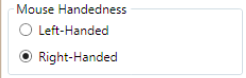
\includegraphics[scale=0.3]{img/GroupBox.png}
\begin{lstlisting}[language=xml]
<GroupBox Header="Mouse Handedness">
    <StackPanel>
        <RadioButton Content="Left-Handed" />
        <RadioButton Content="Right-Handed"
            IsChecked="True"/>
    </StackPanel>
</GroupBox>
\end{lstlisting}
\paragraph{Expander} ermöglicht das Ein und Ausblenden von Infos bei Bedarf. Er wird oft für Zusatzinformationen gebraucht.
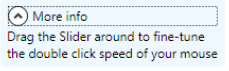
\includegraphics[scale=0.3]{img/expander.png}
\begin{lstlisting}[language=xml]
<Expander>
    <Expander.Header>More info</Expander.Header>
    <TextBlock TextWrapping="Wrap" Text="Drag ..." />
</Expander>
\end{lstlisting}
\paragraph{TabControl} teilt das UI in mehrere Seiten auf. Jedes \code{TabItem} enthält ein eigenes Layout. Das Header Attribut kann mit beliebigem Layout gefüllt werden.
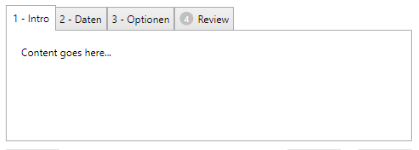
\includegraphics[scale=0.3]{img/tabcontrol.png}
\begin{lstlisting}[language=xml]
<TabControl>
    <TabItem Header="1 - Intro">
        <Grid Margin="10">
        ...
        </Grid>
    </TabItem>
    <TabItem Header="2 - Daten" />
    <TabItem Header="3 - Optionen" />
    <TabItem>
        <TabItem.Header>
            <StackPanel Orientation="Horizontal">
                <Grid>
                    <Ellipse Fill="Silver" Width="16"
                        Height="16" />
                    <Label Content="4" FontSize="10"
                        Foreground="White" />
                </Grid>
            <TextBlock Text="Review" />
            </StackPanel>
        </TabItem.Header>
    </TabItem>
</TabControl>
\end{lstlisting}
\paragraph{Eigene Controls} Es gibt zwei Arten von Controls. Das \code{UserControl} welches als \textbf{Komposition} implementiert wird. Es ist eine Wiederverwendbare Zusammenstellung mehrer COntrols als Gruppe und besteht aus einem XAML und Code-Behind. Es kann nicht mit Styles/Templates umgehen.\\
Das \code{CustomControl} ist eine Ableitung der zu verändernden Klasse. Es erweitert ein bestehendes Control um neue Funktionen. Es besteht aus einem Code-File und ggf. aus einem Standart-Style. Es kann mit Styles/Templates umgehen.



\subsection{Data Grid}

\begin{lstlisting}[language=xml]
<DataGrid ItemsSource="{Binding Customers}"
    AutoGenerateColumns="False" >
  <DataGrid.Columns>
    <DataGridTextColumn Header="First Name" 
        Binding="{Binding FirstName}" />
  </DataGrid.Columns>
  <DataGrid.Columns>
    <DataGridTemplateColumn Header="Image" Width="SizeToCells" 
        IsReadOnly="True">
      <DataGridTemplateColumn.CellTemplate>
        <DataTemplate>
          <Image Source="{Binding Image}" />
        </DataTemplate>
      </DataGridTemplateColumn.CellTemplate>
    </DataGridTemplateColumn>
  </DataGrid.Columns>
</DataGrid>
\end{lstlisting}

\subsection{Package URI}
\begin{itemize}
    \item \code{siteOfOrigin}: relativ zum aktuellen Ordner
    \item \code{application}: relativ zum Assembly
\end{itemize}


